% !TeX program = xelatex 
%% 
%% Copyright 2019-2021 Elsevier Ltd
%% 
%% This file is part of the 'CAS Bundle'.
%% --------------------------------------
%% 
%% It may be distributed under the conditions of the LaTeX Project Public
%% License, either version 1.2 of this license or (at your option) any
%% later version.  The latest version of this license is in
%%    http://www.latex-project.org/lppl.txt
%% and version 1.2 or later is part of all distributions of LaTeX
%% version 1999/12/01 or later.
%% 
%% The list of all files belonging to the 'CAS Bundle' is
%% given in the file `manifest.txt'.
%% 
%% Template article for cas-dc documentclass for 
%% double column output.

\documentclass[a4paper,fleqn,twocolumn]{cas-dc}



% If the frontmatter runs over more than one page
% use the longmktitle option.

%\documentclass[a4paper,fleqn,longmktitle]{cas-dc}

%\usepackage[numbers]{natbib}
%\usepackage[authoryear]{natbib}
\usepackage[authoryear,longnamesfirst]{natbib}

%\usepackage[numbers]{natbib}
%\usepackage[authoryear]{natbib}
%\usepackage[authoryear,longnamesfirst]{natbib}
\usepackage{dsfont}
\usepackage{array}
\usepackage{float}
\usepackage{placeins}
\usepackage{makecell} % add by shuyun
%\usepackage[utf8]{inputenc}
\usepackage{lineno,hyperref}
\usepackage{amsmath}
\usepackage{graphicx}
\usepackage[small]{caption}
\usepackage{subcaption}
\usepackage{array}
\usepackage{multirow}
\usepackage{multicol}
\usepackage{diagbox}
\usepackage{mathrsfs}
\usepackage{color}
\usepackage{booktabs}
\usepackage{soul}
\usepackage{mathspec}
\usepackage{xeCJK}
%

%\setCJKmainfont{STKaiti}

%\setCJKmainfont[Mapping=tex-text]{STKaiti}
\usepackage[ruled, linesnumbered, vlined]{algorithm2e}

%\linenumbers
%%%Author macros
\def\tsc#1{\csdef{#1}{\textsc{\lowercase{#1}}\xspace}}
\tsc{WGM}
\tsc{QE}


\newcommand{\1}[1]{\mathds{1}\left[#1\right]}
\renewcommand{\floatpagefraction}{0.8}

\newcommand{\secref}[1]{Section \ref{#1}}
\newcommand{\figref}[1]{Figure \ref{#1}}
\newcommand{\eqnref}[1]{Eq. (\ref{#1})}
\newcommand{\exref}[1]{Example \ref{#1}}
\newcommand{\algoref}[1]{Algorithm \ref{#1}}
\newcommand{\tableref}[1]{Table \ref{#1}}
\newcommand{\socvec}{SocVec}
\newcommand{\argmin}{\operatornamewithlimits{argmin}}
\newcommand{\argmax}{\operatornamewithlimits{argmax}}
\newtheorem{example}{Example}
\newtheorem{lemma}{Lemma}
\newtheorem{definition}{Definition}
\newcommand{\cut}[1]{}
\newcommand{\ZY}[1]{\textcolor{red}{Zhiyi: #1}}

\begin{document}
%	\begin{multicols}{2}
\let\WriteBookmarks\relax
\def\floatpagepagefraction{1}
\def\textpagefraction{.001}

% Short title
\shorttitle{Empowering Multi-Span Question Answering with Expansive Information Injection using Large Language Models}    

% Short author
\shortauthors{Z. Luo et al.}  

% Main title of the paper
\title{Empowering Multi-Span Question Answering with Expansive Information Injection using Large Language Models}  

\author{Zhiyi Luo}[type=editor,auid=000,bioid=1,orcid=0000-0002-2206-1926]
\ead{luozhiyi@zstu.edu.cn}
\ead[url]{http://zhiyiluo.site}
%\credit{Conceptualization of this study, Methodology, Software}

\author{Yingying Zhang}
\ead{272831920@qq.com}

\author{Ying Zhao}
\ead{272831920@qq.com}

\author{Shuyun Luo}
\cormark[1]
\cortext[mycorrespondingauthor]{Corresponding author}
\ead{shuyunluo@zstu.edu.cn}
\cormark[1]
\cortext[mycorrespondingauthor]{Corresponding author}

\address[mymainaddress]{School of Computer Science and Technology and the Key Laboratory of Intelligent Textile and Flexible Interconnection of Zhejiang Province, Zhejiang Sci-Tech University}
\address[mysecondaryaddress]{No. 928, No. 2 street, Baiyang street, Qiantang New District, Hangzhou 310018, China}


%\Title{Empowering Multi-Span Question Answering with Expansive Information Injection using Large Language Models}
%
%% MDPI internal command: Title for citation in the left column
%\TitleCitation{Title}
%
%% Author Orchid ID: enter ID or remove command
%\newcommand{\orcidauthorA}{0000-0002-2206-1926} % Add \orcidA{} behind the author's name
%%\newcommand{\orcidauthorB}{0000-0000-0000-000X} % Add \orcidB{} behind the author's name
%
%
%% Authors, for the paper (add full first names)
%\Author{Zhiyi Luo $^{1}$\orcidA{}, Yingying Zhang$^{1}$ and Shuyun Luo $^{1,}$*}
%
%%\longauthorlist{yes}
%
%% MDPI internal command: Authors, for metadata in PDF
%\AuthorNames{Zhiyi Luo, Yingying Zhang and Shuyun Luo}
%
%% MDPI internal command: Authors, for citation in the left column
%\AuthorCitation{Luo, Z.; Zhang, Y.; Luo, S.}
%% If this is a Chicago style journal: Lastname, Firstname, Firstname Lastname, and Firstname Lastname.
%
%% Affiliations / Addresses (Add [1] after \address if there is only one affiliation.)
%\address{%
%$^{1}$ \quad School of Computer Science and Technology and the Key Laboratory of Intelligent Textile and Flexible Interconnection of Zhejiang Province, Zhejiang Sci-Tech University, Hangzhou, China; luozhiyi@zstu.edu.cn
%%$^{2}$ \quad Affiliation 2; e-mail@e-mail.com
%}
%
%% Contact information of the corresponding author
%\corres{Correspondence: shuyunluo@zstu.edu.cn;}

% Current address and/or shared authorship
%\firstnote{Current address: Affiliation 3.} 
%\secondnote{These authors contributed equally to this work.}
% The commands \thirdnote{} till \eighthnote{} are available for further notes

%\simplesumm{} % Simple summary

%\conference{} % An extended version of a conference paper

% % Here goes the abstract
\maketitle


\begin{abstract}
	Multi-span question answering has gained prominence as it aligns more closely with real-world user requirements compared to single-span question answering. The utilization of pretrained language models has shown promise in improving multi-span question answering, particularly for factoid questions that necessitate entity-based answers. However, existing methods tend to overlook critical information regarding answer span boundaries, resulting in limited accuracy when generating descriptive answers. To address this limitation, we propose TOAST, a novel joint learning framework specialized in token-based neighboring transitions that capture answer span boundaries through adjacent word relations. Our approach extracts high-quality multi-span answers and is general-purpose, applicable to both alphabet languages like English and logographic languages like Chinese. Furthermore, we introduce CLEAN, a comprehensive open-domain Chinese multi-span question answering dataset, which includes a substantial number of descriptive questions. 
	Extensive experiments demonstrate the superior performance of TOAST over previous top-performing QA models in terms of both EM F1 and overlapped F1 scores. Specifically, the TOAST models, leveraging  $\text{BERT}_{base}$ and $\text{RoBERTa}_{base}$, achieve substantial  improvements in EM F1 scores, with increments of 3.03/2.13, 4.82/3.73, and 16.26/11.53, across three publicly available datasets, respectively. 
\end{abstract}

% Keywords
\begin{keywords}
	Reading comprehension \sep Multi-span question answering \sep  Pretrained language models \sep Multitask learning  \sep Chinese datasets 
\end{keywords}



%%%%%%%%%%%%%%%%%%%%%%%%%%%%%%%%%%%%%%%%%%

\section{Introduction}
\label{sec:intro}

Let's cite a paper~\cite{DBLP:conf/aaai/PangLGXSC19}.

In summary, the main contributions in this paper are as follows:
\begin{itemize}
	\item We employs a automatic data augmentation framework using Large Language Model \((LLM)\) as a knowledge source and a extra content supplement to linearize relevant information and possible continuation from LLM as texts, then inject them into original contexts. 
	\item We develop a series of prompt templates designed for interacting with ChatGPT to acquire comprehensive explanations of numerous entities. These templates ensure that the formats of the responses provided by ChatGPT are highly parseable and well-structured.
	
\end{itemize}

%The introduction should briefly place the study in a broad context and highlight why it is important. It should define the purpose of the work and its significance. The current state of the research field should be reviewed carefully and key publications cited. Please highlight controversial and diverging hypotheses when necessary. Finally, briefly mention the main aim of the work and highlight the principal conclusions. As far as possible, please keep the introduction comprehensible to scientists outside your particular field of research. Citing a journal paper \cite{ref-journal}. Now citing a book reference \cite{ref-book1,ref-book2} or other reference types \cite{ref-unpublish,ref-communication,ref-proceeding}. Please use the command \citep{ref-thesis,ref-url} for the following MDPI journals, which use author--date citation: Administrative Sciences, Arts, Econometrics, Economies, Genealogy, Humanities, IJFS, Journal of Intelligence, Journalism and Media, JRFM, Languages, Laws, Religions, Risks, Social Sciences, Literature.
%%%%%%%%%%%%%%%%%%%%%%%%%%%%%%%%%%%%%%%%%%
\section{Related Work}
\label{sec:related}
In this section, we briefly summarize previous works that are relevant to extractive reading comprehension
(RC) datasets and various modeling approaches employed for extractive RC tasks.
\subsection{Multi-Span RC Datasets}
The complete answer to a real-world user question could consist of multiple text spans. 
Furthermore, a user question can even have multiple intents, where the answer to each intent is composed of one or more spans. 
We refer to the datasets focus on such multi-span questions as multi-span RC datasets.
Natural Question~\citep{DBLP:journals/tacl/KwiatkowskiPRCP19} and Quoref~\citep{DBLP:conf/emnlp/DasigiLMSG19} both contain multi-span questions. 
The Natural Question dataset incorporates real anonymized queries to the Google search engine. 
Quoref is used to validate models with the ability to resolve co-reference among entities. %, which is not for general capability validation of models.
However, the proportion of multi-span answers in Natural Question and Quoref is relatively low, around 2\% and 10\% respectively. 
The DROP~\citep{DBLP:conf/naacl/DuaWDSS019} dataset which consists of complex questions on history and football games, requires discrete reasoning over the content of contexts, including  co-reference resolution and arithmetic operations, such as addition, sorting and counting. 
Although the questions could be multi-span, the answer spans are almost exclusively semantically homogeneous and related to numeric values. 
MASH-QA~\citep{DBLP:conf/aaai/PangLGXSC19} is a domain-specific dataset that extends the answer space to general text types in the healthcare domain.
Recently, \cite{li2022multispanqa} propose the MultiSpanQA dataset, which consists of open-domain multi-span questions. The MultiSpanQA dataset is derived from Natural Question, whose questions are real queries issued to the Google search engine. 
Each question is associated with a context extracted from a retrieved Wikipedia page.  
MultiSpanQA also has an expanded variant by introducing single-span and unanswerable questions, namely MultiSpanQA (expand). 

\subsection{Neural Models for RC}
Research in reading comprehension grows rapidly, and many successful neural-based RC models have been proposed in this area. 
%As discussed in \secref{sec:related_dataset}, the extractive RC datasets support to cast RC as answer extraction task.
Typically, neural  models~\citep{DBLP:conf/aaai/PangLGXSC19,DBLP:conf/iclr/Wang017a,DBLP:conf/iclr/XiongZS17} for RC are composed of two components, a context encoder and an answer decoder. 
The context encoder is used to encode the information of questions, contexts and their interactions in-between. Then, the answer decoder aims to generate the answer texts based on outputs of the context encoder. 
To make the answer decoder compatible with the answer extraction task, 
Pointer Network~\citep{DBLP:conf/nips/VinyalsFJ15} model has been adopted to
% tackle the problem that 
%generates answer texts from contexts. 
copy tokens from the given contexts as answers~\citep{DBLP:conf/acl/KadlecSBK16,DBLP:conf/emnlp/TrischlerYYBSS16}.
\cite{DBLP:conf/iclr/Wang017a} proposed a boundary model, which utilized Pointer Network to predict the start and end indices for an answer span.
%\ZY{single token - single span - multispan}
%Boundary Model
\cite{DBLP:conf/iclr/SeoKFH17} proposed an alternative way for the implementation of answer decoder, that built neural position classifiers upon the encoder outputs, predicting the start and end indices of the answer span in the context.

% neural layer unifies the components of encoder and decoder together that 
Recently, the RC models upgrade the context encoder using pre-trained language models (PrLMs)~\citep{radford2018improving,kenton2019bert,liu2019roberta,lee2020biobert,gu2021domain} 
%such as GPT~\citep{radford2018improving}, BERT~\citep{kenton2019bert} and RoBERTa~\citep{liu2019roberta}
, benefiting from the invention of Transformer~\citep{vaswani2017attention} blocks.
%Benefiting from nowadays pretrained language models (PrLMs) based on Transformer~\cite{vaswani2017attention} blocks, recent RC models upgrades the context encoder using PrLMs such as BERT. 
%the context encoder and answer decoder can be unified into a standard algorithm that utilize PrLMs such as BERT to encode inputs, then predict the start position and end position for the answer span.
\cite{DBLP:conf/naacl/DevlinCLT19}  proposed a standard extractive model for  single-span RC that utilizes BERT to encode inputs, then builds position classifiers to predict where the answer span starts and ends.
However, the answer decoder, whether implemented with Pointer Network or position classifiers, predicts start and end position independently, thus can not distinguish the different answer spans properly.
%Pang et al. proposed HAS-QA~\cite{} which built the conditional pointer network and aggregators to model multiple answer spans.
~\cite{DBLP:conf/emnlp/ZhuAJ0R20} proposed MultiCo which used a contextualized sentence selection method to capture the relevance among multiple sentence-based answer spans in order to form an answer with multiple sentences.
%However, such single-span extractive model is not suitable for multi-span RC task which can be formulated as multi-span extraction.
These models are not well adapted to multi-span RC which can be formulated as more flexible task of multi-span extraction where each span can be a word, phrase, sentence or any continuous string of text.

%the start position and end position of the answer span. 
%PrLMs unify the context encoder and answer decoder as a standard algorithm, that  
%\subsubsection{Single-span Models}
%~\citep{yoon2022,DBLP:journals/corr/abs-2302-01691} 
Extracting a variable number of spans from an input text can be commonly cast as a sequence tagging problem.
\cite{segal2020simple} proposed using a sequence tagging model for multi-span extraction, which predicts whether each token is part of an answer. \cite{yoon2022} employed a similar sequence tagging approach to address extractive question answering~\citep{DBLP:journals/bmcbi/NaseemDKK22}  in the biomedical domain.
\cite{li2022multispanqa} also adopted the tagging model architecture, integrating two sub-tasks: predicting the number of spans to extract and annotating the answer structure within their proposed dataset to capture global information.
ADRAV~\citep{hu2023biomedical} proposed a dynamic routing and answer voting method to further make full use of the hidden layer knowledge of pre-trained models.
More recently, LIQUID~\citep{lee2023liquid} was introduced to  automatically generate list-style QA pairs from unlabeled corpora. LIQUID extracted named entities from the summarized text as candidate answers and incorporated synthetic data in the tagging model. 
These methods harness the extensive factual knowledge embedded in powerful contextualized encoders (PrLMs) or synthesized data that resolves around named entities. 
As a result, they have demonstrated promising performance in extracting  multi-span answers, particularly for factoid questions where the answers correspond entities.
%Benefiting from the rich factual knowledge implied in the powerful contextualized encoders (PrLMs) or synthesized data centered around name entities, these methods have achieved promising performance on multi-span answer extraction, especially for factoid questions where the answers are entities.
%These methods have been achieved promising performance on multi-span answer extraction, especially for factoid questions whose answers are entities, benefiting from the rich factoid knowledge implied in the powerful context encoder like PrLMs.
However, these methods do not take into account the information of span boundaries in terms of the questions, and thus have very limited capabilities of precisely drawing a description answer. 
%However, for these methodswhich are implied in the powerful context encoder like PrLMs, they are failed to care span boundaries .
Compared to these approaches, TOAST incorporates the semantic and syntactic information of span boundaries by explicitly modeling the implicit neighboring transitions in-between the adjacent tokens or words, which benefits the span boundary identification.


\subsection{Interaction with LLMs}



%%%%%%%%%%%%%%%%%%%%%%%%%%%%%%%%%%%%%%%%%%
\section{Our Approach}

	\begin{figure*}[h]
	\centering
	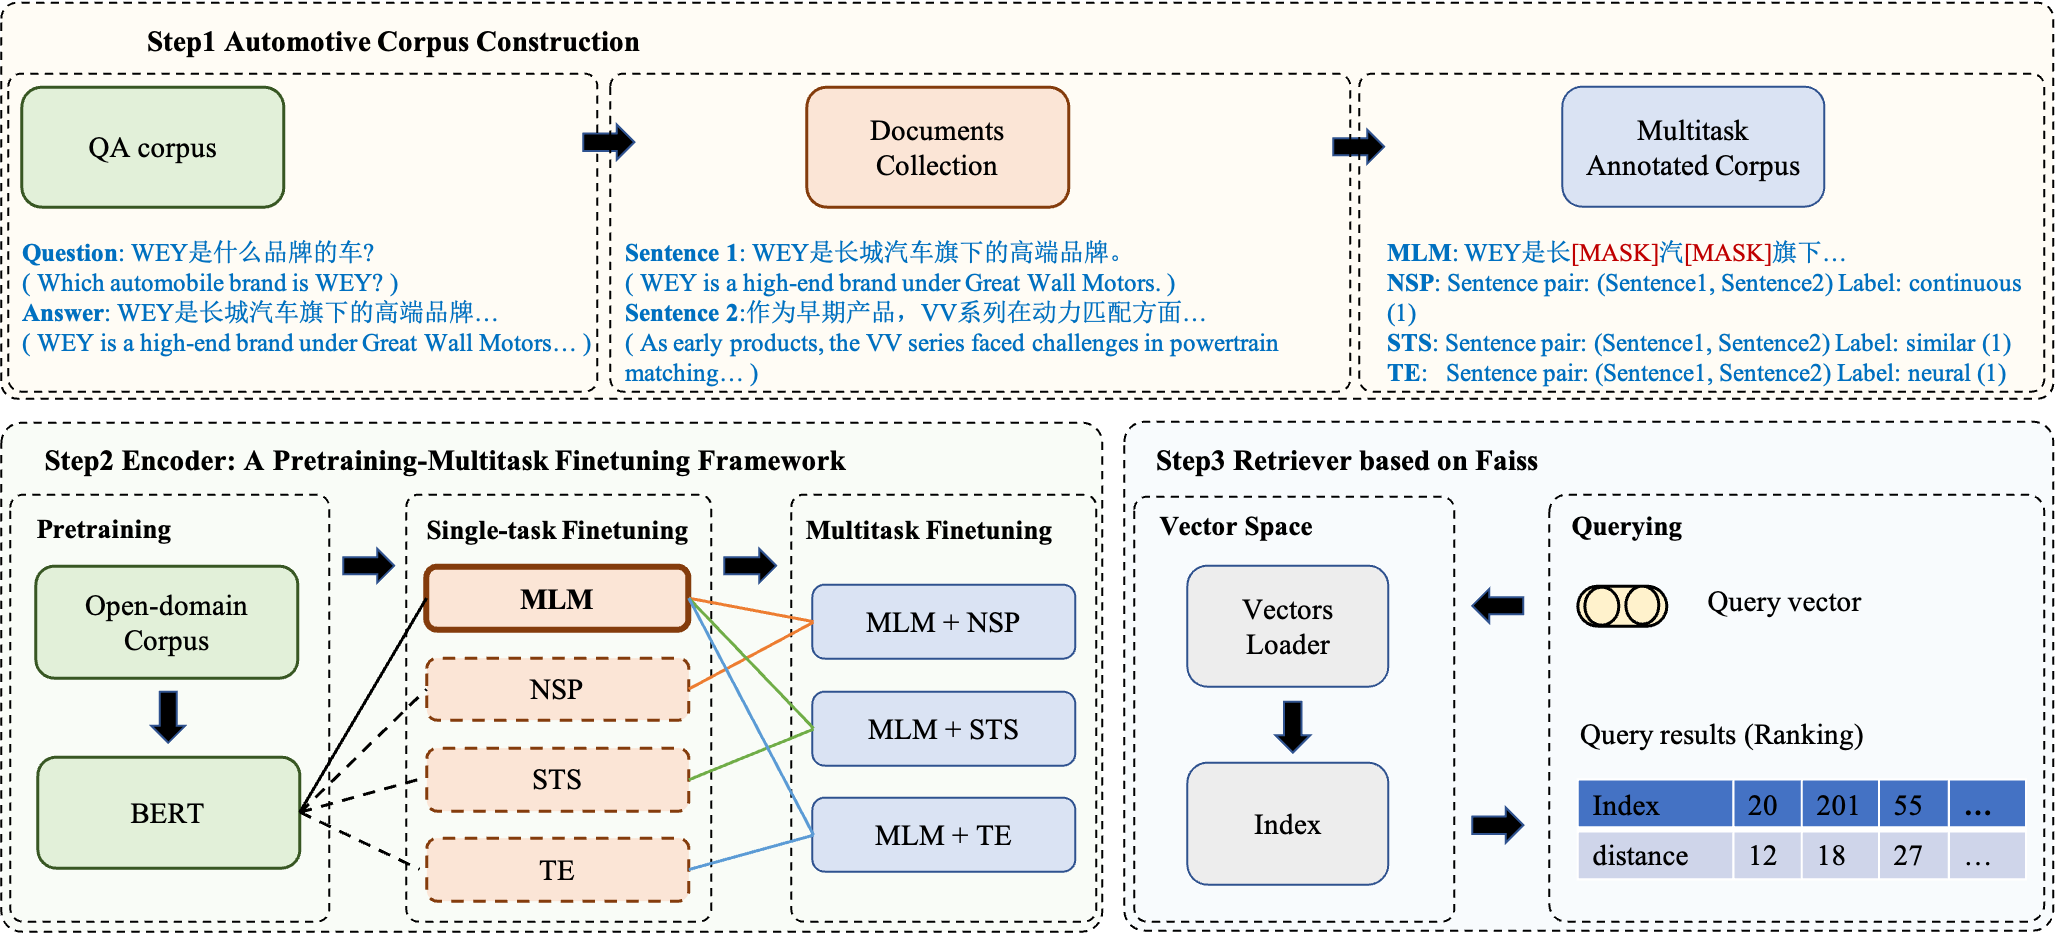
\includegraphics[width=18cm]{overview.png}
	\caption{An overview of our automatic information augmentation framework. \textbf{(a) Step 1}: Interact with ChatGPT to Get Auxiliary Information. \textbf{(b) Step 2}: Distilling the Information and Injecting Them into Context \textbf{(c) Step 3}: Input the Augmented Context into Tagging Model}
	\label{fig:overview}
	\end{figure*}   


%\unskip
	Existing extractive multi-span question answering models exhibit subpar performance in handling ambiguous words, complex proper nouns (such as film and song titles), numerical values, and long descriptive answers. The main reasons for these shortcomings can be categorized into three aspects:
	
	\textbf{Ambiguous Words}: The real world is replete with words that have a single form but multiple meanings, which heavily depend on the context. For instance, the word ``Cameron" could refer to a famous director or a former British Prime Minister, depending on the context. The specific meanings of such words often appear infrequently in training corpora, making them difficult to learn.
	
	\textbf{Numerical Values}: In contrast to ambiguous words, numerical values have a single meaning but can be represented in various forms. For example, "22.5 billion years" can also be expressed as "cosmic years".
	
	\textbf{Multi-span Answers}: In extractive multi-span question answering tasks, the model needs to grasp the overall relationship of multi-span answers in the context, such as parallelism and progression.These challenges require the model to possess a high level of comprehensive understanding ability and knowledge about language and the world. 
	
	Leveraging large language models to parse question-answering data and inject auxiliary knowledge into the model can promote the integration of the model's latent world knowledge and specific domain knowledge in the paragraph, thereby enhancing the model's performance. Thus, we use GPT-3.5-turbo to generate entity annotations, entity association analysis, and content continuation for each question-answering paragraph as auxiliary information for the model:
	
	\textbf{Context Supplementary}: By inserting explanations of entities in the form of annotations after the main entities or concept words in the question and paragraph, this method helps the model capture the actual meaning of ambiguous words in specific contexts. It provides direct information prompts for low-frequency meanings or low-frequency words, achieving entity or concept alignment in the question-answering system.
	
	\textbf{Context Enrichment}: By integrating entity association analysis and content continuation with the original question-answering text to form new paragraphs based on knowledge enhancement, this method captures the inherent associations between words or entity concepts with the same meaning but different forms. On one hand, it parses the logical relationships between other entities using entity relationship analysis. On the other hand, it extends the original paragraph information using content continuation, introducing more external knowledge while helping the model understand the overall content direction of the paragraph, thereby enhancing the model's comprehension ability.

	
	Overall,we design an automated knowledge enhancement method for multi-span question answering tasks, which interacts with large language models based on templates. This method is applicable to all question answering models or frameworks. It is universally applicable to any other downstream tasks that contain paragraph data, without the need for any complex calculations. In the following sections, we will provide a detailed introduction to each specific module of this process.

\subsection{Construction of Prompt Template}
	\label{sec:prompt_construction}
	\begin{figure*}[h]
		\centering
		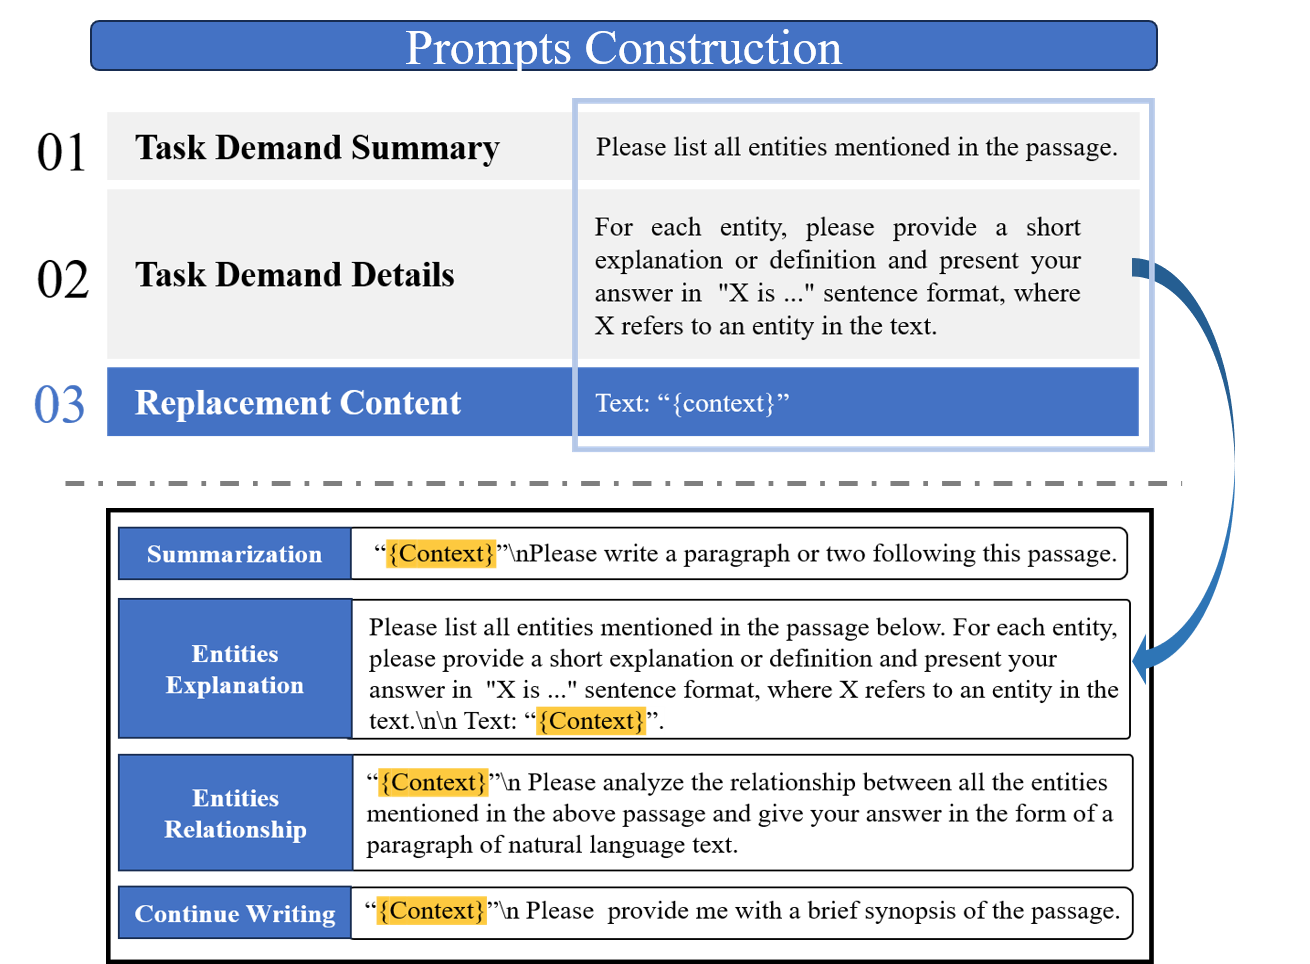
\includegraphics[width=14.5cm]{Prompts_construction.png}
		\caption{Prompt Templates and it's Construction}
		\label{fig:prompt_template}
	\end{figure*}   
	
	The quality and format of the content produced by LLMs depends greatly on the prompts. Hence, it is necessary to clarify the format and content requirements of the outputs in advance, and to refine the templates that meet the expectations through extensive evaluation.
	For entity relationship parsing and textual continuation, it would be better to ensured that the the output is a natural paragraph, to facilitate the automatic splicing of the enriched knowledge with the initial paragraphs,which is consistent with encoder's natural input format.
	Regarding knowledge of entity explanation, the inserted knowledge fusion method requires a parsable and structured outputs for automatic recognition and segmentation of entities and their explanations in post-processing, as well as inserting explanation behind the description of matched entity in initial context.
	
	Concretely, by clearly specifying the form and requirements in the prompts, especially for entity relationship parsing and contextual continuation, which need to be formulated in the form of natural statements, the targeted enhanced knowledge can be obtained more easily.
	Furthermore, to obtain well-structured results for complex model interactions, like entity explanations, we utilize a set of corresponding hint templates to construct the process, which has proven to be useful for interactions that require semi-structured answers through verification. 
	
	Eventually, the template is piloted to clarify any ambiguous requirements in the template to confirm an accurate understanding of the LLMs (e.g., adding at the end of the prompt, ``Please return the answer in the following form, being careful not to repeat it: \textbackslash n\textbackslash nA is .....")  In addition, to avoid omission or confusion of requirements due to the length of the prompt text, specific principles should be reiterate in a separate paragraph.
	
\subsection{Information Injection}

	To incorporate enhanced knowledge into the original data (comprising questions and paragraphs) pertaining to entity interpretation, a methodology involving the insertion of explanations is employed. Specifically, the process begins with the automated script parsing of entity interpretation data. This script, on one hand, utilizes regular expressions to analyze the structure of the majority of sentences, while on the other hand, for a limited subset of sentences that deviate from the template specifications, employs Spacy's Semantic Dependency Analysis model to identify entities and their corresponding interpretations.
	
	Upon obtaining the ``Entity-Entity Interpretation" knowledge base for each question-and-answer data, a subsequent scan of the original context is conducted. For each entity that exists in the dataset's library of entities and their explanations, the corresponding explanation is inserted immediately following the entity, enclosed within parentheses. This meticulous approach ensures that the augmented text, enriched with knowledge, retains its natural sentence or paragraph flow. For instance, a resulting sentence might appear as follows: ``How long does it take for the Milky Way (Milky Way: The galaxy that contains our Solar System and is home to billions of stars.) to rotate?" 
	
	\label{sec:information_injection}
	\begin{figure*}[h]
		\centering
		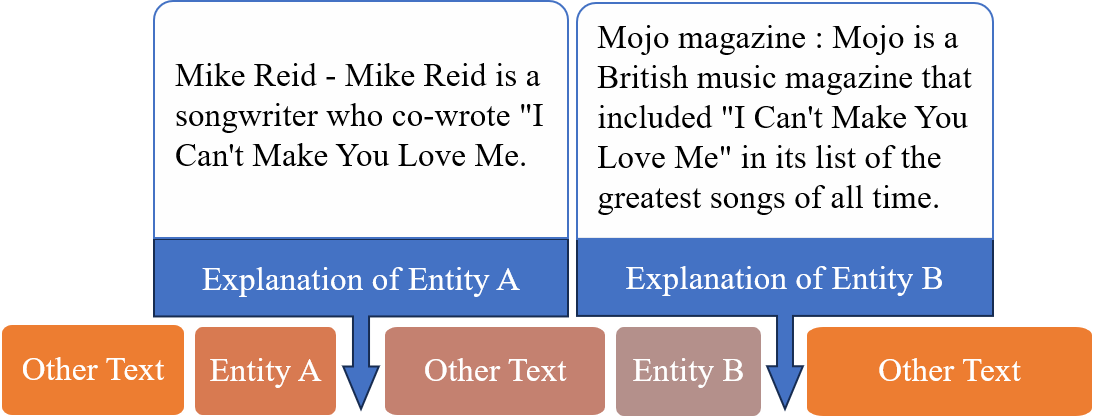
\includegraphics[width=10cm]{EntityInsert.png}
		\caption{The Process of Inserting Entity Explanation into Context}
		\label{fig:entity_insertion}
	\end{figure*}

	For the incorporation of enhanced knowledge related to entity relationship analysis and content continuation, a method of random slicing and concatenation based on length ratios is employed to infuse the augmented knowledge into the original paragraphs. Initially, the ratio of the average length of the augmented knowledge text to that of the original paragraph is calculated. Subsequently, at the model's input layer, the original input data is segmented into text fragments of length of \textit{512 * average original length / (average original length + average augmented text length)}, and the augmented text is also segmented into text fragments of length of  \textit{512 * average augmented text length / (average original length + average augmented text length)}. Then, random selections of augmented text fragments are made and concatenated into the middle of each original text fragment. Finally, this concatenated longer text is fed into the model in a sliding manner to ensure comprehensive interaction between the original data and the augmented data at lower layers of the model, as illustrated in Figure~\ref{fig:random_concatenate}.
   


\begin{figure*}[h]
	\centering
	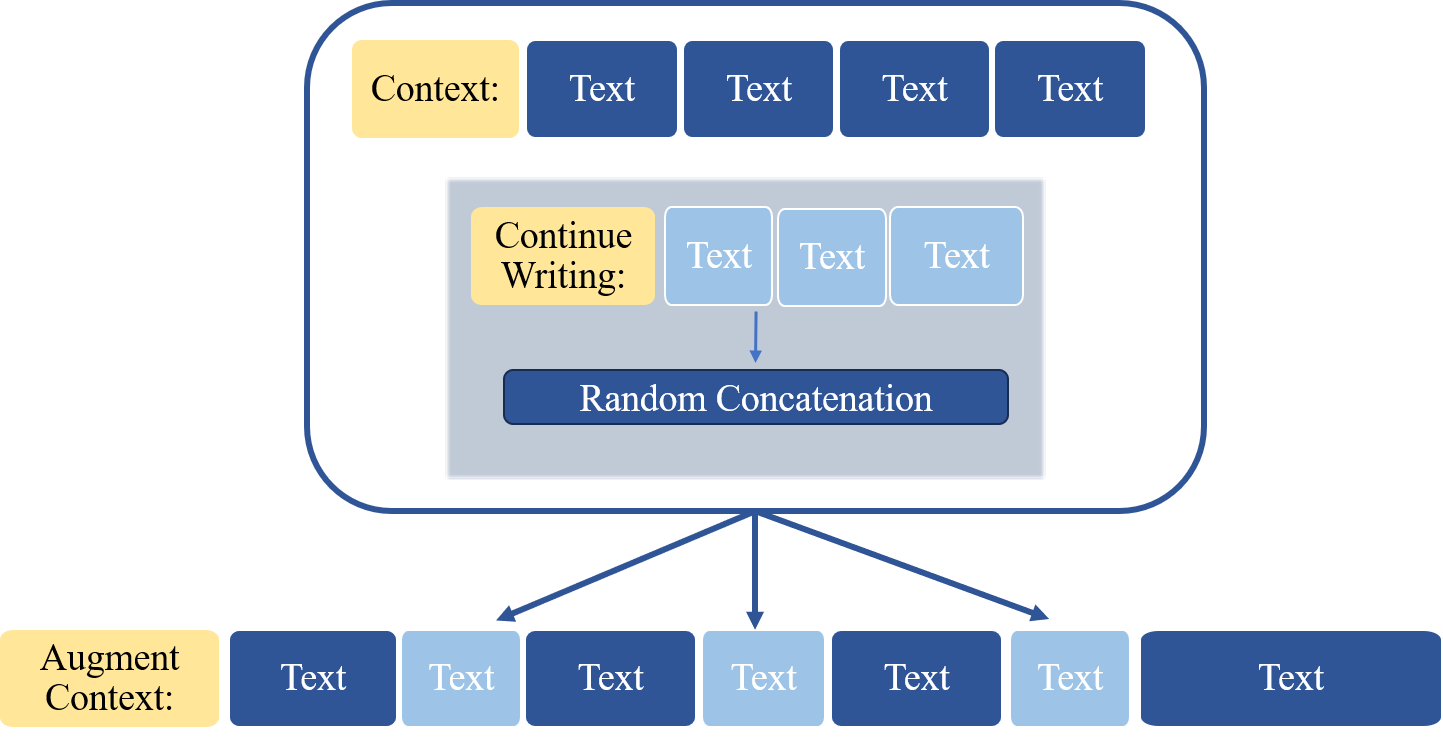
\includegraphics[width=10cm]{RandomConcat.png}
	\caption{The Process of Concatenation of Original Context and Auxiliary Information}
	\label{fig:random_concatenate}
\end{figure*}  

\subsection{Information Integration}
\label{sec:information_integration}
	In addition to the aforementioned three types of information, we seek more valuable enhanced information by requesting summaries for each question-context pair from Large Language Models (LLMs). We then extract entities mentioned in the summaries to capture those highly relevant to the core context. Moreover, recognizing the intrinsic connection between entity explanation and entity relationship parsing, we categorize them as complementary information for context enrichment, with context continuation serving as supplementary information. This approach aims to augment the model's internal text-parsing knowledge with external world knowledge through enhanced information. 
	
	To further investigate the efficacy of multi-information integration, leveraging enhanced information derived from Large Language Models (LLMs), we employ two distinct approaches to combine entity knowledge and context continuity. The first approach involves the incorporation of all information within the original context, with each type of information undergoing individualized knowledge injection. The second approach, referred to as "bagging," treats models trained on diverse information sources as voters. For each query, we employ all model predictions for token-level BIO labeling within the context, determining the final prediction through a majority vote. In cases of tie-breaking, we prioritize the logits' magnitude to ascertain the ultimate prediction.
	

\section{Experiments}
In this section, we compare our information augmentation approach with multiple strong baseline on multi-span question answering. We first introduce the datasets and experiment setup, then show the experimental results and analysis for different model.

\subsection{Evaluation Dataset}
\label{sec:datasets}
	 We conducted experiments on MultiSpanQA(Li et al., 2022), a recently introduced Reading Comprehension dataset designed for multi-span question answering. This dataset comprises 6.5K multi-span examples in which the questions represent user queries issued to the Google search engine, and the contexts are extracted from the English Wikipedia. It's worth noting that there is a expand variant of MultiSpanQA known as MultispanQA(expand), which intakes single-span and answerable questions. However, we did not perform a comparison with the expanded dataset due to its relatively lower proportion of multi-span QA pairs.

\subsection{Experimental Setup}
	For all competing models and our model, we use the HuggingFace implementation of $\text{BERT}_{base}$ or $\text{RoBERTa}_{base}$ as the \textit{encoder} with $\textit{max\_len}$ = 512. We set the initial learning rate as $3 \times 10^{-5}$ and  $\textit{batch\_size}$ = 4, and use the BERTAdam optimizer with a weight decay of 0.01. Our approach does not involve tuning the parameters on the validation set. Instead, we rely on the model checkpoints obtained after 5 epochs. Next, we introduce the comparison model and evaluation metrics in our experiments.
	
	\subsubsection{\textit{Model Under Comparison}}
	\label{sec:baselines}
	We introduce two comstracting models approaches to multi-span answer extraction : \textbf{TASE} (Segal et al., 2020) and \textbf{LIQUID}(Lee et al., 2023). TASE utilizes a tag-based span extraction model which identifies multi-span answers though the assigning a tag to every input token with BIO tagging scheme. On the other hand, LIQUID serves as a framework for generating multi-span QA datasets to improve model performance.
	
	To enhance the context with auxiliary information, we employ two distinct   approaches: \textbf{$\text{AUG}_{c}$} and \textbf{$\text{AUG}_{eree}$}, where \textbf{AUG} is our automatic data augmentation framework,and the suffix indicates which kind of information is injected into the context. \textbf{$\text{AUG}_{C}$} enriches the context with continue writing, while \textbf{$\text{AUG}_{EREE}$} supplements context with entities information including explanation and relationship analysis.
	Specifically, we leverage ChatGPT as a knowledge source to linearize the relevant information from large language models. in texts format and seamlessly integrate into the original contexts, thus reinforces the information of model inputs.

	
	\subsubsection{\textit{Evaluation Metrics}}
	\label{sec:metrics}
	We use two automatic metrics for evaluation: Exact Match and Overlap F1 score.
	\begin{itemize}
		\item \textbf{Exact Match}. An exact match occurs when a predicted span fully matches one of the ground-truth
		answer spans. We calculate the micro-average precision, recall and f1 score for the extract match
		metric.
		
		\item \textbf{Overlap F1 score}. Overlap F1 score is the macro-average f1 score, where the f1 score for each
		example is computed by treating the prediction and gold as a bag of tokens.
	\end{itemize}


\subsection{Experimental Results and Analysis}
	In this section, we compare $\text{AUG}$ with all competing models described above quantitatively.
	
	\subsubsection{\textit{Comparison Results}}
	We evaluate our model as well as baselines 
	\(( Section ~\ref{sec:baselines} )\) on the development splits of multi-span datasets \(( Section  ~\ref{sec:datasets})\) using automatic metrics \(( Section ~\ref{sec:datasets})\). The comparison results are shown in Table \ref{tab:bertall}, Table \ref{tab:robertaall}.
	
	\begin{table*}[width=\textwidth,cols=9,pos=h]  % 
		\caption{Approach performance on complete MultiSpanQA valid set based on $\text{BERT}_{base}$.} 
		\label{tab:bertall}
		\begin{tabular*}{\textwidth}{@{\extracolsep{\fill}}lccccccc}
			\toprule
			\multirow{2}{*}{\textbf{Model}} & \multicolumn{3}{c}{Exact Match} & \multicolumn{3}{c}{Partial Match}  \\
			\cline{2-7} 
			\addlinespace
			& F\((\%)\) & P\((\%)\) & R\((\%)\) & F\((\%)\) & P\((\%)\) & R\((\%)\) \\
			\midrule
			TASE   & 60.28 & 55.59 & 65.83 & 78.16 & 78.27 & 78.06 \\ 
			LIQUID & 61.44 & 58.39 & 64.84 & 78.56 & 78.65 & 78.46 \\
			$\text{AUG}_{c}$ & 63.05 & 58.51 & 68.34 & 79.42 & 78.70 & 80.14 \\
			$\text{AUG}_{eree}$  & 63.93 & 60.22 & 68.13 & 77.50 & 77.07 & 77.94 \\
			$\text{AUG}_{ereec}$ & 62.90  & 61.02 & 64.89 & 76.72 & 78.56 & 74.97 \\
			Bagging & 64.44 & 61.63 & 67.50 & 79.5 & 80.49 & 78.57 \\
			\bottomrule
		\end{tabular*}
		%	\noindent{\footnotesize{\textsuperscript{1} Tables may have a footer.}}
	\end{table*}
	
	\begin{table*}[width=\textwidth,cols=8,pos=h]  
		\caption{Approach performance on complete MultiSpanQA valid set based on $\text{RoBERTa}_{base}$.} 
		\label{tab:robertaall}
		\begin{tabular*}{\textwidth}{@{\extracolsep{\fill}}lccccccc}
			\toprule
			\multirow{2}{*}{\textbf{Model}} & \multicolumn{3}{c}{Exact Match} & \multicolumn{3}{c}{Partial Match}  \\
			\cline{2-7} 
			\addlinespace
			& F\((\%)\) & P\((\%)\) & R\((\%)\) & F\((\%)\) & P\((\%)\) & R\((\%)\) \\
			\midrule
			TASE & 68.00 & 65.06 & 71.22 & 83.13 & 83.05 & 83.22 \\ 
			LIQUID & 68.33 & 66.68 & 70.07 & 82.71 & 82.45 & 82.98 \\
			$\text{AUG}_{c}$ & 70.35 & 67.35 & 73.63 & 84.06 & 83.38 & 84.76 \\
			$\text{AUG}_{eree}$ & 69.15 & 67.81 & 70.54 & 82.85 & 83.90 & 81.83 \\
			$\text{AUG}_{ereec}$ & 70.44 & 67.83 & 73.26 & 82.80 & 82.45 & 83.15 \\
			Bagging & 70.86 & 69.03 & 72.79 & 84.82 & 85.53 & 84.12 \\
			\bottomrule
		\end{tabular*}      
		%	\noindent{\footnotesize{\textsuperscript{1} Tables may have a footer.}}
	\end{table*}
	Table~\ref{tab:bertall} and Table~\ref{tab:robertaall} illustrate the performance comparison between the proposed approaches, $\text{AUG}_{c}$ and $\text{AUG}_{eree}$, and several strong baselines, including the previous state-of-the-art model LIQUID. These comparisons are conducted using both the $\text{BERT}_{base}$ and $\text{RoBERTa}_{base}$ encoders, and regard multi-span question answering as a \textit{BIO} sequence tagging task to predict each token whether it is a part or begin of an answer. 
	Notably,$\text{AUG}_{c}$ exhibit superior performance across the evaluate dataset on all metrics. However, on Partial Match scores, $\text{AUG}_{eree}$ demonstrates slightly lower performance compared to TASE, and especially lower than LIQUID when employing the $\text{BERT}_{base}$ encoder.
	Importantly, the performance of $\text{AUG}_{c}$ consistently outperforms LIQUID and TASE on all metrics and encoders, irrespective of the encoder setting.
	These results demonstrate the effectiveness of our proposed framework, as well as the efficacy of the information augmentation strategy.
	 
	To be more specific, Table~\ref{tab:bertall} shows comparisons of metrics among all competing models 100 backed by $\text{BERT}_{base}$. We can see that our proposed framework, AUG, consistently outperforms all other baselines across multispanQA dataset. Backed by $\text{BERT}_{base}$, $\text{AUG}_{c}$ achieves EM and Overlap F1 scores of 63.05 and 79.42, respectively. Moreover, when equipped with entities’ information,  $\text{AUG}_{eree}$ achieves even higher EM F1 scores of 63.93 but relatively lower Overlap F1 of 77.50 than baselines on the same encoder. These results showcase substantial improvements over the previous state-of-the-art model, LIQUID, with EM F1 score enhancements ranging from 1.61 to 2.49 percents across validation datasets. 
	
	Additionally, when utilizing $\text{RoBERTa}_{base}$ instead of $\text{BERT}_{base}$, $\text{AUG}_{c}$ achieves EM and Overlap F1 scores of 70.35 and 84.06 respectively on the same datasets. These scores represent EM and Overlap F1 improvements of 2.02 and 0.93 compared to the previous setup. For  $\text{AUG}_{eree}$, the EM F1 score represents an enhancement of 0.82, with the EM and Overlap F1 values of 69.16 and 82.85 respectively. Notably, the partial metrics also indicate lower values compared to TASE and LIQUID, in line with the result supported by $\text{BERT}_{base}$. This is because augmenting the model with entity information, including definition and relationship knowledge, strengthens its ability to capture and understand entity concepts, which leads the model to prefer complete entity spans or empty span set as answers rather than partial entity span, and therefore a decrease in the partial recall and ultimately a lower partial F1 scores and a higher EM F1.
	

	To further substantiate our explanation for the suboptimal performance of our model on the Overlap F1 metric, we conducted a detailed examination of the predictions made by $\text{AUG}_{eree}$ and two baseline models on the validation dataset. In essence, we tallied the instances where these models predicted empty answers and recalculated their Overlap F1 scores on non-empty predictions. This allowed us to investigate whether the $\text{AUG}_{eree}$ model aligns with our hypothesis, which posits that its extensive learning of entity knowledge during training makes it inclined to output either a complete and accurate answer span or no answer at all, as opposed to a partially correct answer span.

	As presented in Table~\ref{tab:answer_counts}, $\text{AUG}_{eree}$ indeed predicted a higher number of empty answers compared to TASE and LIQUID, while achieving relatively higher Overlap F1 scores on non-empty predictions. Specifically, when equipped with $\text{BERT}_{base}$ as the encoder, $\text{AUG}_{eree}$ obtained an F1 score of 0.7976 on non-empty answer predictions, whereas TASE and LIQUID scored 0.7964 and 0.7909, respectively. With $\text{RoBERTa}_{base}$, $\text{AUG}_{eree}$ achieved an Overlap F1 score of 0.8414, surpassing TASE and LIQUID, which scored 0.8404 and 0.8357, respectively. Additionally, it is worth noting that $\text{AUG}_{eree}$ consistently predicted more empty answers, whether using BERT or RoBERTa.

	These findings lend support to our conjecture that the introduction of entity knowledge leads to a slight reduction in the model's Overlap F1 scores. This suggests that utilizing LLM as a knowledge source to linearize entity information from LLM text and integrate it into the original context empowers the model to acquire greater entity knowledge, thereby exhibiting a preference for more accurate and complete answer spans, or simply providing no answer.
	
	
	
		\begin{table*}[width=\textwidth,cols=9,pos=h]  % 
		\caption{The statistics of answers span predicted by $\text{AUG}_{eree}$ and baselines} 
		\label{tab:answer_counts}
		\begin{tabular*}{\textwidth}{@{\extracolsep{\fill}}lccccccc}
			\toprule
			\multirow{2}{*}{\textbf{ }} & \multicolumn{3}{c}{$\text{BERT}_{base}$} & \multicolumn{3}{c}{$\text{RoBERTa}_{base}$}  \\
			\cline{2-7} 
			\addlinespace
			& TASE\((\%)\) & LIQUID\((\%)\) & $\text{AUG}_{eree}$\((\%)\) & TASE\((\%)\) & LIQUID\((\%)\) & $\text{AUG}_{eree}$\((\%)\) \\
			\midrule
			empty predictions counts   & 0.0245 & 0.0214 & \textbf{0.0643} & 0.0061 & 0.0153 & \textbf{0.0291} \\ 
			non-empty Overlap f1  & 0.7964 & 0.7909 & \textbf{0.7976} & 0.8404 & 0.8357 & \textbf{0.8414} \\
			\bottomrule
		\end{tabular*}
		%	\noindent{\footnotesize{\textsuperscript{1} Tables may have a footer.}}
		\end{table*}
	
	
	
	Totally, the result, displayed in Table~\ref{tab:robertaall} demonstrates the same trends to Table~\ref{tab:bertall}. And the outcome highlights robustness in effectively generalizing across different datasets without requiring hyperparameter re-tuning. 
	
\subsubsection{\textit{Discussion}}
	Table~\ref{tab:bertall} and Table~\ref{tab:robertaall} discuss the performance of different augmentation integrated strategies, including the results-bagging methods whose outputs are voting results of $\text{AUG}_{c}$, $\text{AUG}_{eree}$ as well as LIQUID, and the input-fusion model $\text{AUG}_{ceree}$ who injects all kinds of information above into input contexts.
	
	In detail, with EM f1 scores of 62.90 and 64.44 in Table~\ref{tab:bertall} and 70.44 and 70.86 in Table~\ref{tab:robertaall}, both the $\text{AUG}_{ceree}$ and Bagging methods consistently surpass TASE and LIQUID, which exhibits robust effectiveness of information injection strategies. However, there is a little decrease caused by fusing all auxiliary information when contrast with single information augmentation strategies and the bagging method. This may be due to the likelihood that incorporating all of the augmentation information into the model inputs will confuse the model by introducing excessive auxiliary knowledge and underrepresented original context proportion. Therefore it may be more useful that adding limit information into context, and using result-bagging method, a multi-model voting to bringing all information into model with an indirect way.
	
	From the Partial Match perspective, $\text{AUG}_{ceree}$ and the Bagging method achieve 76.72 and 79.52 in Table~\ref{tab:bertall}, and 82.80 and 84.82 in Table~\ref{tab:robertaall}. In accordance with Exact Match metrics, Bagging demonstrate a overall superior performance. Meanwhile overlap f1 score of $\text{AUG}_{eree}$ is inferior to TASE but superior to LIQUID ,with relatively higher precision and relativelv higher recall, which  is comparable to all single augmented models such as $\text{AUG}_{eree}$. And its weak performance on overlap f1 also reveals complete entities preference of this information injection approach.
	
	Furthermore, we stratified the data within MultispanQA according to answer types, specifically categorizing them into DESC, NUM, and ENTYS. We subsequently conducted a comparative analysis of model performance within each of these subcategories. In particular, the results are presented in Tables~\ref{tab:bertsub} and Table~\ref{tab:robertasub}, supported by $\text{BERT}_{base}$ and $\text{RoBERTa}_{base}$, respectively.
	As indicated in Tables~\ref{tab:bertsub} and~\ref{tab:robertasub}, our proposed models exhibit superior performance in terms of EM F1 scores for all categorizing. However, they demonstrate suboptimal performance in terms of overlap F1 scores.
	

	
	\begin{table*}[ht]
		\caption{Model performance on complete MultiSpanQA valid Subset with different answer types based on $\text{BERT}_{base}$.}
		\label{tab:bertsub}
		\begin{tabular*}{\textwidth}{@{\extracolsep{\fill}}lccccccc}
			\toprule
			\multirow{2}{*}{\textbf{Type}} & \multirow{2}{*}{\textbf{Model}} & \multicolumn{3}{c}{Exact Match} & \multicolumn{3}{c}{Partial Match} \\
			\cmidrule{3-8} 
			& & F\((\%)\) & P\((\%)\) & R\((\%)\) & F\((\%)\) & P\((\%)\) & R\((\%)\) \\
			\midrule
			\multirow{6}{*}{DESC} & TASE & 32.76 & 27.33 & 40.87 & 64.46 & 68.61 & 60.79 \\ 
			& LIQUID & 36.69 & 31.10 & 44.71 & 66.05 & 65.95 & 66.15 \\
			& $\text{AUG}_{c}$ & 38.74 & 32.89 & 47.12 & 68.31 & 70.32 & 66.42 \\
			& $\text{AUG}_{eree}$ & 44.69 & 40.71 & 49.52 & 63.12 & 67.16 & 59.53 \\
			& $\text{AUG}_{ereec}$ & 40.63 & 38.30 & 43.27 & 64.25 & 71.15 & 58.57 \\
			& Bagging & 39.91 & 36.69 & 43.75 & 66.70 & 73.68 & 60.93 \\
			\midrule
			\multirow{6}{*}{NUM} & TASE & 33.33 & 30.23 & 37.14 & 60.98 & 71.99 & 52.89 \\ 
			& LIQUID & 34.33 & 31.25 & 38.10 & 60.68 & 68.15 & 54.69 \\
			& $\text{AUG}_{c}$ & 35.96 & 33.33 & 39.05 & 64.47 & 71.56 & 58.65 \\
			& $\text{AUG}_{eree}$ & 36.20 & 34.48 & 38.10 & 59.02 & 65.63 & 53.62 \\
			& $\text{AUG}_{ereec}$ & 36.71 & 37.25 & 36.19 & 57.09 & 69.04 & 48.67 \\
			& Bagging & 35.94 & 34.82 & 37.14 & 60.73 & 71.15 & 52.97 \\
			\midrule
			\multirow{6}{*}{ENTYS} & TASE & 66.30 & 62.21 & 70.96 & 81.16 & 80.37 & 81.96 \\ 
			& LIQUID & 67.17 & 65.25 & 69.21 & 81.66 & 81.69 & 81.63 \\
			& $\text{AUG}_{c}$ & 68.47 & 64.44 & 73.03 & 81.93 & 80.57 & 83.34 \\
			& $\text{AUG}_{eree}$ & 68.36 & 64.64 & 72.53 & 80.55 & 79.21 & 81.93 \\
			& $\text{AUG}_{ereec}$ & 67.54 & 65.60 & 69.59 & 79.49 & 80.16 & 78.83 \\
			& Bagging & 69.65 & 66.94 & 72.59 & 82.31 & 82.07 & 82.55 \\
			\bottomrule
		\end{tabular*}
	\end{table*}
	
	\begin{table*}[ht]
		\caption{Model performance on complete MultiSpanQA valid Subset with different answer types based on $\text{RoBERTa}_{base}$.}
		\label{tab:robertasub}
		\begin{tabular*}{\textwidth}{@{\extracolsep{\fill}}lccccccc}
			\toprule
			\multirow{2}{*}{\textbf{Type}} & \multirow{2}{*}{\textbf{Model}} & \multicolumn{3}{c}{Exact Match} & \multicolumn{3}{c}{Partial Match} \\
			\cmidrule{3-8} 
			& & F\((\%)\) & P\((\%)\) & R\((\%)\) & F\((\%)\) & P\((\%)\) & R\((\%)\) \\
			\midrule
			\multirow{6}{*}{DESC} & TASE & 45.53 & 40.84 & 51.44 & 75.44 & 76.61 & 74.31 \\ 
			& LIQUID & 48.68 & 44.76 & 53.37 & 73.27 & 71.57 & 75.04 \\
			& $\text{AUG}_{c}$ & 49.02 & 44.66 & 54.33 & 76.33 & 77.85 & 74.86 \\
			& $\text{AUG}_{eree}$ & 50.99 & 46.96 & 55.77 & 76.87 & 78.07 & 75.71 \\
			& $\text{AUG}_{ereec}$ & 49.24 & 44.71 & 54.81 & 71.87 & 73.03 & 70.74 \\
			& Bagging & 47.70 & 43.78 & 52.40 & 77.43 & 80.63 & 74.47 \\
			\midrule
			\multirow{6}{*}{NUM} & TASE & 46.23 & 45.79 & 46.67 & 71.89 & 78.42 & 66.36 \\ 
			& LIQUID & 40.19 & 39.45 & 40.95 & 67.56 & 72.28 & 63.42 \\
			& $\text{AUG}_{c}$ & 50.69 & 49.11 & 52.38 & 72.86 & 80.22 & 66.74 \\
			& $\text{AUG}_{eree}$ & 42.40 & 41.07 & 43.81 & 66.67 & 73.51 & 61.00 \\
			& $\text{AUG}_{ereec}$ & 45.58 & 44.55 & 46.67 & 65.86 & 73.19 & 59.87 \\
			& Bagging & 44.65 & 43.64 & 45.71 & 70.11 & 78.49 & 63.35 \\
			\midrule
			\multirow{6}{*}{ENTYS} & TASE & 72.57 & 69.94 & 75.41 & 84.90 & 84.32 & 85.48 \\ 
			& LIQUID & 72.95 & 71.77 & 74.16 & 85.02 & 84.75 & 85.29 \\
			& $\text{AUG}_{c}$ & 74.59 & 71.87 & 77.53 & 85.79 & 84.40 & 87.23 \\
			& $\text{AUG}_{eree}$ & 73.50 & 72.81 & 74.22 & 84.74 & 85.49 & 83.99 \\
			& $\text{AUG}_{ereec}$ & 75.04 & 72.81 & 77.41 & 85.37 & 84.46 & 86.29 \\
			& Bagging & 75.85 & 74.52 & 77.22 & 86.73 & 86.73 & 86.74 \\
			\bottomrule
		\end{tabular*}
	\end{table*}

\subsubsection{\textit{Ablation Experiment}}
	At the end of this section, we conducted ablations on our approach to confirm the effectiveness of selecting the information injection proportion. For each QA data, we randomly split the original context and the auxiliary text, then concatenated them into a final augmented context with a specific proportion to ensure that the new input length meets $\textit{max\_len}$, which has a crucial impact on our approach. In practice, we determined the final text splicing ratio by calculating the ratio of the average length of the source text to the added information, which for the $\text{AUG}_{c}$ is 0.86.
	
	Specifically, Table~\ref{tab:different_ratio_bert} and Table~\ref{tab:different_ratio_roberta} displays $\text{AUG}_{c}$'s performance with differential proportion to concatenate original contexts and continuation, on complete MultispanQA valid set,backed by $\text{BERT}_{base}$ and $\text{RoBERTa}_{base}$ respectively. We choose five proportions for information integration, which determine how much auxiliary information would be inject into each overflowed text segment. The results presented in tables indicate that using the ratio of their average lengths as the proportion of the overflow text composed of original text and auxiliary information is an effective approach. In detail, $\text{AUG}_{c}$,equipping with $\text{BERT}_{base}$, achieves an Exact Match F1 scores improvements of at least 4.57 compared to other proportions and an overlap F1 scores improvements of at least 2.07. In line with Table~\ref{tab:different_ratio_bert}, when $\text{AUG}_{c}$ equips with $\text{Roberta}_{base}$, it achieves an improvement of Exact Match F1 scores of 0.55 but an decrease of Overlap F1 scores of 0.17.



\begin{table*}[H] 
	\caption{Ablations of $\text{AUG}_{c}$ on different proportion for information concatenation, based on $\text{BERT}_{base}$.} 
	\label{tab:different_ratio_bert}
	\newcolumntype{C}{>{\centering\arraybackslash}X}
	\begin{tabular*}{\textwidth}{@{\extracolsep{\fill}}lccccccc}
		\toprule
		\multirow{2}{*}{\textbf{Proportion}} & \multicolumn{3}{c}{Exact Match} & \multicolumn{3}{c}{Partial Match}  \\
		\cline{2-7} 
		\addlinespace
		& F\((\%)\) & P\((\%)\) & R\((\%)\) & F\((\%)\) & P\((\%)\) & R\((\%)\) \\
		\midrule
		0.90 & 58.55 & 57.69 & 59.44 & 71.88 & 74.30 & 69.61 \\ 
		0.70 & 61.70 & 59.03 & 64.63 & 76.58 & 77.84 & 75.36 \\
		0.50 & 61.22 & 57.37 & 65.62 & 77.38 & 77.61 & 77.16 \\
		0.40 & 61.36 & 56.50 & 67.13 & 78.26 & 77.57 & 78.96 \\
		0.10 & 61.41 & 56.36 & 67.45 & 78.94 & 78.45 & 79.44 \\
		0.14 & 63.05 & 58.51 & 68.34 & 79.42 & 78.70 & 80.14 \\
		\bottomrule
	\end{tabular*}      
	%	\noindent{\footnotesize{\textsuperscript{1} Tables may have a footer.}}
\end{table*}



\begin{table*}[H] 
	\caption{Ablations of $\text{AUG}_{c}$ on different proportion for information concatenation, based on $\text{RoBERTa}_{base}$.} 
	\label{tab:different_ratio_roberta}
	\newcolumntype{C}{>{\centering\arraybackslash}X}
	\begin{tabular*}{\textwidth}{@{\extracolsep{\fill}}lccccccc}
		\toprule
		\multirow{2}{*}{\textbf{Proportion}} & \multicolumn{3}{c}{Exact Match} & \multicolumn{3}{c}{Partial Match}  \\
		\cline{2-7} 
		\addlinespace
		& F\((\%)\) & P\((\%)\) & R\((\%)\) & F\((\%)\) & P\((\%)\) & R\((\%)\) \\
		\midrule
		0.90 & 58.13 & 56.92 & 59.39 & 71.70 & 73.49 & 69.98 \\ 
		0.70 & 66.97 & 65.42 & 68.60 & 80.05 & 80.80 & 79.32 \\
		0.50 & 68.94 & 67.23 & 70.75 & 82.43 & 83.23 & 81.64 \\
		0.40 & 68.95 & 66.11 & 71.06 & 83.71 & 83.71 & 81.71 \\
		0.10 & 69.80 & 66.47 & 73.47 & 84.23 & 83.49 & 84.99 \\
		0.86 & 70.35 & 67.35 & 73.63 & 84.06 & 83.38 & 84.76 \\
		\bottomrule
	\end{tabular*}      
	%	\noindent{\footnotesize{\textsuperscript{1} Tables may have a footer.}}
\end{table*}



%\begin{table}[H] 
%	\caption{Ablations of $\text{AUG}_{c}$ on different proportion for information concatenation, based on $\text{BERT}_{base}$.} 
%	\label{tab:different_ratio_roberta}
%	\newcolumntype{C}{>{\centering\arraybackslash}X}
%	\begin{tabularx}{\textwidth}{p{1.7cm}CCCCCCC}
%		\toprule
%		\multirow{2}{*}{\textbf{Proportion}} & \multicolumn{3}{c}{Exact Match} & \multicolumn{3}{c}{Partial Match}  \\
%		\cline{2-7} 
%		\addlinespace
%		& F\((\%)\) & P\((\%)\) & R\((\%)\) & F\((\%)\) & P\((\%)\) & R\((\%)\) \\
%		\midrule
%		0.90 & 58.13 & 56.92 & 59.39 & 71.70 & 73.49 & 69.98 \\ 
%		0.70 & 66.97 & 65.42 & 68.60 & 80.05 & 80.80 & 79.32 \\
%		0.50 & 68.94 & 67.23 & 70.75 & 82.43 & 83.23 & 81.64 \\
%		0.40 & 68.95 & 66.11 & 71.06 & 83.71 & 83.71 & 81.71 \\
%		0.10 & 69.80 & 66.47 & 73.47 & 84.23 & 83.49 & 84.99 \\
%		0.86 & 70.35 & 67.35 & 73.63 & 84.06 & 83.38 & 84.76 \\
%		\bottomrule
%	\end{tabularx}      
%	%	\noindent{\footnotesize{\textsuperscript{1} Tables may have a footer.}}
%\end{table}
%
%\section{Conclusion}


%All figures and tables should be cited in the main text as Figure~\ref{fig1}, Table~\ref{tab1}, etc.

%\section{Discussion}
%
%Authors should discuss the results and how they can be interpreted from the perspective of previous studies and of the working hypotheses. The findings and their implications should be discussed in the broadest context possible. Future research directions may also be highlighted.

%%%%%%%%%%%%%%%%%%%%%%%%%%%%%%%%%%%%%%%%%%
%\section{Conclusions}
%
%This section is not mandatory, but can be added to the manuscript if the discussion is unusually long or complex.


%%%%%%%%%%%%%%%%%%%%%%%%%%%%%%%%%%%%%%%%%%
\vspace{6pt} 

%%%%%%%%%%%%%%%%%%%%%%%%%%%%%%%%%%%%%%%%%%
%% optional
%\supplementary{The following supporting information can be downloaded at:  \linksupplementary{s1}, Figure S1: title; Table S1: title; Video S1: title.}

% Only for journal Methods and Protocols:
% If you wish to submit a video article, please do so with any other supplementary material.
% \supplementary{The following supporting information can be downloaded at: \linksupplementary{s1}, Figure S1: title; Table S1: title; Video S1: title. A supporting video article is available at doi: link.}

% Only for journal Hardware:
% If you wish to submit a video article, please do so with any other supplementary material.
% \supplementary{The following supporting information can be downloaded at: \linksupplementary{s1}, Figure S1: title; Table S1: title; Video S1: title.\vspace{6pt}\\
%\begin{tabularx}{\textwidth}{lll}
%\toprule
%\textbf{Name} & \textbf{Type} & \textbf{Description} \\
%\midrule
%S1 & Python script (.py) & Script of python source code used in XX \\
%S2 & Text (.txt) & Script of modelling code used to make Figure X \\
%S3 & Text (.txt) & Raw data from experiment X \\
%S4 & Video (.mp4) & Video demonstrating the hardware in use \\
%... & ... & ... \\
%\bottomrule
%\end{tabularx}
%}

%%%%%%%%%%%%%%%%%%%%%%%%%%%%%%%%%%%%%%%%%%
%\authorcontributions{For research articles with several authors, a short paragraph specifying their individual contributions must be provided. The following statements should be used ``Conceptualization, X.X. and Y.Y.; methodology, X.X.; software, X.X.; validation, X.X., Y.Y. and Z.Z.; formal analysis, X.X.; investigation, X.X.; resources, X.X.; data curation, X.X.; writing---original draft preparation, X.X.; writing---review and editing, X.X.; visualization, X.X.; supervision, X.X.; project administration, X.X.; funding acquisition, Y.Y. All authors have read and agreed to the published version of the manuscript.'', please turn to the  \href{http://img.mdpi.org/data/contributor-role-instruction.pdf}{CRediT taxonomy} for the term explanation. Authorship must be limited to those who have contributed substantially to the work~reported.}

%=====================================
% References, variant A: external bibliography
%=====================================
%\bibliography{your_external_BibTeX_file}

\section*{Acknowledgements}
This research was supported by the Natural Science Foundation of Zhejiang Province, China (Grant No. LQ22F020027), Fundamental Research Funds of Zhejiang Sci-Tech University (Grant No. 23232138-Y), Liaoning Provincial Natural Science Foundation of China (Grant No. 2022-KF-21-01) and the Key Research and Development Program of Zhejiang Province, China (Grant No. 2023C01041 and 2022C01079).

\bibliographystyle{cas-model2-names}
% 
\bibliography{refs}
%\end{multicols}
\end{document}

